\documentclass[12pt,letterpaper]{article}

%Note to Self:
%When Decommission? - after two months of feeling useless or right away?

\usepackage[utf8]{inputenc}
\usepackage[letterpaper,margin=1in]{geometry}
\usepackage{caption} % for table captions

\usepackage{amsmath} % for multi-line equations and piecewises
\usepackage{indentfirst} % to indent after a section
\usepackage{setspace}
\usepackage{times}
\usepackage{graphicx}
\usepackage{textcomp}
\usepackage{xspace}
\usepackage{verbatim} % for block comments
\usepackage{subfig} % for subfigures
\usepackage{enumitem} % for a) b) c) lists
\newcommand{\Cyclus}{\textsc{Cyclus}\xspace}%
\newcommand{\Cycamore}{\textsc{Cycamore}\xspace}%
\usepackage{tabularx}
\usepackage{color}
\definecolor{bg}{rgb}{0.95,0.95,0.95}
\newcolumntype{b}{X}
\newcolumntype{s}{>{\hsize=.5\hsize}X}
\newcolumntype{m}{>{\hsize=.75\hsize}X}
\usepackage{titling}
\usepackage[newfloat]{minted}

\newenvironment{code}{\captionsetup{type=listing}}{}
\SetupFloatingEnvironment{listing}{name=Code}

\newcommand{\subtitle}[1]{%
  \posttitle{%
    \par\end{center}
    \begin{center}\large#1\end{center}
    \vskip0.5em}%
}
\usepackage{tikz}


\usetikzlibrary{shapes.geometric,arrows}
\tikzstyle{process} = [rectangle, rounded corners, minimum width=3cm, minimum height=1cm,text centered, draw=black, fill=blue!30]
\tikzstyle{arrow} = [thick,->,>=stealth]


\graphicspath{{images/}}
 
\usepackage[font={footnotesize,it}]{caption}
 



\setlength{\parindent}{15pt} % Default is 15pt.




\fontfamily{ptm}\selectfont

\title{Numerical Experiments for Verifying Demand Driven Deployment Algorithms}
\author{Jin Whan Bae and Gwendolyn Chee}
\date{2017-10-11}


\begin{document}
	
	\maketitle
	\hrule
	\onehalfspacing
	\thispagestyle{empty}

\section{Introduction}
For many fuel cycle simulations, it is currently up to the user to define
a deploy scheme, or facility parameters, to make sure that there's no gap
in the supply chain. Or, the same goal is achieved by setting the
\texttt{facility} capacity to infinity, which does not reflect real-world
conditions. 

The Demand-Driven Cycamore Archetype project (NEUP-FY16-10512) aims to develop \Cycamore demand-driven deployment capabilities.
The developed algorithm, in the form of \Cyclus \texttt{Institution}
agent, deploys \texttt{facilities} to meet the front-end and back-end demand of the 
fuel cycle.

This report provides numerical tests for non-optimizing, deterministic-optimizing and stochastic-optimizing prediction algorithms.

These prediction models are being developed by the University of South Carolina. 
In this report, we discuss numerical experiments for testing the non-optimizing, 
deterministic optimizing and stochastic optimizing methods. The numerical 
experiments will be designed for both the once through nuclear fuel 
cycle and advanced fuel cycles. 


\section{Method}
This report lists necessary capabilities of the new \Cyclus \texttt{institute}
for demand-driven deployment of fuel cycle facilities. 
Then the report lists tests to check correct implementation of the capabilities,
with a sample fuel cycle with well-defined facility parameters.


\section{Configuration}
The user defines prototypes to be deployed for fuel facilities,
and reactor deployment scheme.  The reactor deployment causes the demand of fuel
which triggers fuel facility deployment. The detailed input file XML input schema
is shown in Appendix A. 


\section{Logic Flow}

The algorithm creates a supply chain with the fuel facilities,
then calculates the demand for each facility. A simple example is illustrated in
figure \ref{diag:dem}.


\begin{figure}[H]
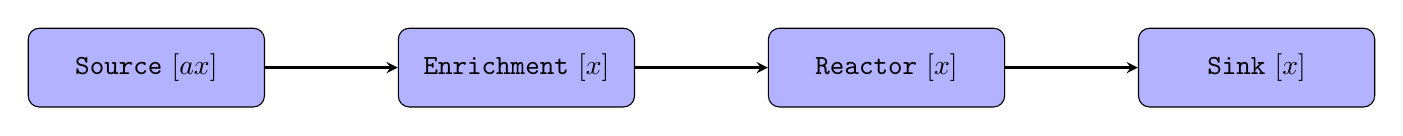
\begin{tikzpicture}[node distance=4.7cm]
\node (source) [process] {\texttt{Source} [$ax$]};
\node (enrichment) [process, right of=source] {\texttt{Enrichment} [$x$]};
\node (reactor) [process, right of=enrichment]{\texttt{Reactor} [$x$]};
\node (sink) [process, right of=reactor]{\texttt{Sink} [$x$]};

\draw [arrow] (source) -- (enrichment); 
\draw [arrow] (enrichment) -- (reactor);
\draw [arrow] (reactor) -- (sink);
\end{tikzpicture}
\caption{Simple flow of materials. The values in the bracket are demands calculated
         by the algorithm. The \texttt{Reactor} demands $x$ amount of fuel,
         which translates into demands of $x$ from \texttt{Enrichment} and \texttt{Sink}.
         The \texttt{Source} has a demand of $a x$ to take in for enrichment losses.
         $a \approx 9 $ in LEU PWRs.}
\label{diag:dem}
\end{figure}

If the demand of a commodity exceeds the current supply, the \texttt{Institution}
builds more facilities to meet the demand for that commodity.


%% This is Where I worked Till %%%%%
%% This is Where I worked Till %%%%%
%% This is Where I worked Till %%%%%
%% This is Where I worked Till %%%%%

\subsection{Reactor Parameters for Test Scenarios}
Table \ref{tab:reactor} provides the parameters for the \texttt{reactors} in the test scenarios and Table \ref{tab:everythingelse} provides the parameters for the \texttt{source}, \texttt{enrichment} and \texttt{sink} facilities in the test scenarios.

\begin{table}[h]
    \centering
    \begin{tabularx}{\textwidth}{bbb}
       \hline
       Reactor Parameters & Value & Units \\
       \hline
       Cycle Time & 2 & timesteps \\
       Refuel Time & 1 & timesteps \\
       Lifetime & 6 & timesteps \\
       Power Capacity & 1000 & MWe \\
       Assembly Size & 100 & kg \\
       \# assemblies per core & 3 & \\
       \# assemblies per batch & 1 & \\
       \hline
    \end{tabularx}
    \caption {Reactor Parameters}
    \label{tab:reactor}
\end{table}

\begin{table}[H]
     \centering
    \begin{tabularx}{\textwidth}{bbb}
       \hline
       Parameters & Value & Units \\
       \hline
       Natural U Composition & 0.71 & \% U235\\
       Tails Assay & 0.003 & \% U235 \\
       Fuel Enrichment & 4 & \% U235 \\
       Enrichment throughput & 300 & $\frac{kg}{month \cdot facility}$ \\
       Enrichment SWU Capacity & 2000 & $\frac{SWU}{month \cdot facility}$ \\
       Source Throughput & 3000 & $\frac{kg}{month \cdot facility}$\\
       Sink Capacity & 200 &  $\frac{kg}{facility}$ \\
       \hline
    \end{tabularx}
    \caption {Source, Enrichment and Sink Facility Parameters}
    \label{tab:everythingelse}
\end{table}

An example input file with the facility and simulation
definitions can be found in the input directory of this repository.

\newpage
\subsection{Non-optimizing prediction method}
To ensure that the non-optimizing prediction model is working correctly, each function of the code must be tested to determine if its output matches the analytical solution. In this section, the tests that must be met is described based on the parameters defined in Table \ref{tab:reactor} and \ref{tab:everythingelse} and analytical solution of a defined simple scenario. Unit test examples are included in Appendix B.
\\
\\
\noindent
\textbf{Test 1: A reactor outputs the user defined power capacity when deployed and does not output
power capacity when decommissioned.} \\
Test Scenario: A single reactor is deployed at time step 3 and decommissioned at time step 5. \\
Analytical Solution: During cycle time, the reactor will have a power output of 1000MWe. Therefore,
there is only be power output of 1000MWe at time steps 3 and 4. The analytical solution of
the power output of the reactor per time step is given in Table \ref{tab:power}.

\begin{table}[H]
     \centering
    \begin{tabularx}{\textwidth}{bbb}
       \hline
       Timestep & Reactor Power Output (MWe) \\
       \hline
       1 & 0 \\
       2 & 0 \\
       3 & 1000 \\
       4 & 1000 \\
       5 & 0 \\
       6 & 0 \\
       \hline
    \end{tabularx}
    \caption {Analytical solution of the power output of the reactor per time step}
    \label{tab:power}
\end{table}

\noindent
\textbf{Test 2: A reactor outputs the user defined power capacity during its cycle time and not during its refuel time.} \\
Test Scenario: A single reactor is deployed at time step 3 and decommissioned at time step 8. \\
Analytical Solution: Based on the reactor parameters defined in Table 1, the reactor will have a cycle time of 2 time steps and a refuel time of 1 time step. Therefore, there is only be power output of 1000MWe during cycle time steps. The analytical solution of the power output of the reactor per time step is given in Table \ref{tab:cycles}.

\begin{table}[H]
     \centering
    \begin{tabularx}{\textwidth}{bbb}
       \hline
       Timestep & Reactor Power Output (MWe) \\
       \hline
       1 & 0 \\
       2 & 0 \\
       3 & 1000 \\
       4 & 1000 \\
       5 & 0 \\
       6 & 1000 \\
       7 & 1000 \\
       8 & 0 \\
       9 & 0 \\
       \hline
    \end{tabularx}
    \caption {Analytical solution of the power output of the reactor per time step}
    \label{tab:cycles}
\end{table}

\noindent
\textbf{Test 3:1 or more of the facility that produces reactor’s input commodity (fuel) is deployed when the amount of fuel available is below the amount of fuel required by the reactor.} \\
Test Scenario: A single reactor is deployed at time step 3.\\
Analytical Solution: Based on the simple supply chain example in Figure 1 and enrichment facility parameters defined in Table 2, an enrichment facility must be deployed at time step 3 to meet fuel demand. The analytical solution of the fuel available per time step is given in Table \ref{tab:fuel}.

\begin{table}[H]
     \centering
    \begin{tabularx}{\textwidth}{bbb}
       \hline
       Timestep & Fuel (kg) \\
       \hline
       1 & 0 \\
       2 & 0 \\
       3 & 300 \\
       4 & 0 \\
       \hline
    \end{tabularx}
    \caption {Analytical solution of the fuel available per time step}
    \label{tab:fuel}
\end{table}



\begin{comment}
\subsubsection{\texttt{Reactor}}
\noindent
\textbf{Condition 1: All the reactors run at full capacity} \\
This is tested by determining the total number of time steps which both \texttt{Reactor}s are in operation, one \texttt{Reactor} is in operation or none is in operation. Based on the values of the analytical solution in Table \ref{tab:poweroutput}, there should be 2 time steps where both 
\texttt{Reactor}s are in operation, 6 time steps where only one \texttt{Reactor} is in operation and 2 time steps where no \texttt{Reactor}s are in operation. 

\noindent
\textbf{Condition 2: A new \texttt{Reactor} is deployed when the energy demand exceeds the energy produced by the current \texttt{Reactor}s} \\
This is tested by comparing the total number of \texttt{Reactor}s deployed to the analytical solution. Based on values of the analytical solution in Table \ref{tab:deployment}, in total 2 \texttt{Reactor}s were deployed.  

\noindent 
\textbf{Condition 3: A \texttt{Reactor} is decommissioned when the energy demand falls behind the output of the current \texttt{Reactor}s}

\subsubsection{\texttt{Enrichment}}
\noindent 
\textbf{Condition 1: The enriched uranium produced by \texttt{Enrichment} is equal to the analytic solution of the enriched uranium required by the \texttt{Reactor} for each time step} \\
This is tested by determining the total number of SWUs produced by the \texttt{Enrichment} facilities. These values are compared to the SWUs produced per time step in the analytical solution in Table \ref{tab:analytical}. 

\noindent
\textbf{Condition 2: A new \texttt{Enrichment} facility is deployed when the enriched uranium required by the \texttt{Fuelfab} exceeds the enriched uranium produced of current \texttt{Enrichment} facilities} \\
This is tested by comparing the total number of \texttt{Enrichment} facilities deployed to the analytical solution. Based on values of the analytical solution in Table \ref{tab:deployment}, in total 2 \texttt{Enrichment} facilities were deployed.

\noindent 
\textbf{Condition 3: A \texttt{Enrichment} facility is decommissioned when the enriched uranium required by the \texttt{Fuelfab} falls behind the enriched uranium produced by current \texttt{Enrichment} facilities}

\subsubsection{\texttt{Source}}
\noindent 
\textbf{Condition 1: The mined uranium produced by \texttt{Source} is equal to the analytical solution of the mined uranium required by the \texttt{Enrichment} facilities for each time step}\\
This is tested by determining the total amount of Uranium mined by the \texttt{Source}. These values are compared to the Uranium produced per time step in the analytical solution in Table \ref{tab:analytical}.

\noindent
\textbf{Condition 2: A \texttt{Source} facility is deployed when mined uranium required by the \texttt{Enrichment} facilities exceeds mined uranium produced by the current \texttt{Source}} \\
This is tested by comparing the total number of \texttt{Source} facilities deployed to the analytical solution. Based on values of the analytical solution in Table \ref{tab:deployment}, in total 2 \texttt{Source} facilities were deployed.

\noindent 
\textbf{Condition 3: A \texttt{Source} facility is decommissioned when mined uranium required by the \texttt{Enrichment} facilities falls behind the mined uranium required by the current \texttt{Source}}


commented out till further time
\subsection{Deterministic-Optimizing/Stochastic prediction method}
The following conditions need to be satisfied for each segment of the fuel cycle. 

\begin{enumerate}
\item Do all the \texttt{Reactor}s run? 
\begin{minted}{c++}
TEST(ReactorTests, DDDeploy_DO) {
    [Example input with the following attributes:]
        [int simdur = 20;]
        [Defines reactor with zero refueling cycle and operation 
        cycle of 1 month]
        [Defines fuel cycle facilities parameters]
        [Defines Reactor Deploy Scheme / Power Demand]
        [Increasing Fuel Demand with Time]
    [Run test]
    [Test if Reactor has no zero values in output Timeseriespower]
}
\end{minted}
\item  Do all the \texttt{Reactor}s run at full capacity (not lacking fuel)? 
\begin{minted}{c++}
TEST(ReactorTests, DDDeploy_DO) {
    [Example input with the following attributes:]
        [int simdur = 20;]
        [Defines reactor with zero refueling cycle, power capacity 
        of x and operation cycle of 1 month]
        [Defines fuel cycle facilities parameters]
        [Defines Reactor Deploy Scheme / Power Demand]
        [Increasing Fuel Demand with Time]
    [Run test]
    [Test if Reactor has x value in output Timeseriespower]
}
\end{minted}

\item Is the objective function optimized?

\item Is the constraint followed? 

\item  Do the related fuel cycle facilities get deployed upon demand?
\begin{minted}{xml}
TEST(ReactorTests, DDDeploy_NO) {
    [Example input with the following attributes:]
        [int simdur = 20;]
        [Defines reactor with zero refueling cycle and operation 
        cycle of 1 month]
        [Defines fuel cycle facilities parameters]
        [Defines Reactor Deploy Scheme / Power Demand]
        [Increasing Fuel Demand with Time]
    [Run test]
    [Test if fuel facility is deployed in the beginning]
    [Test if fuel facility is deployed later in the simulation 
    (have analytic solution)]
}
\end{minted}

\item Do the related fuel cycle facilities exit upon demand decrease?
\begin{minted}{xml}
TEST(ReactorTests, DDDeploy_NO) {
    [Example input with the following attributes:]
        [int simdur = 20;]
        [Defines reactor with zero refueling cycle and operation 
        cycle of 1 month]
        [Defines fuel cycle facilities parameters]
        [Defines Reactor Deploy Scheme / Power Demand]
        [Decreasing Fuel Demand with Time]
    [Run test]
    [Test if fuel facility is deployed in the beginning]
    [Test if fuel facility exits later in the simulation (have 
    analytic solution)]
}
\end{minted}


\end{enumerate}



\section{Advanced Fuel Cycles}
\end{comment}

\section{Appendix A - parameter configuration}

First, the user defines the prototypes to be deployed
to support the reactor.

\begin{code}

\begin{minted}[bgcolor=bg]{xml}
<interleave>
  <element name="institution">
    <data type="string"/>
  </element>
    <element name="prototypes">
      <oneOrMore>
        <element name="val">
          <data type="string"/>
        </element>
      <oneOrMore>
    </element>
</interleave>

\end{minted}
\captionof{listing}{Fuel cycle facility prototype definition}
\label{code:pro}
\end{code}


Then deployment of the power-producing reactors is defined, and the user
is given two choices:
\begin{itemize}
  \item Manually define the deployment scheme of reactors (code \ref{code:man_reac})
  \item Define power demand equation (code \ref{code:fun_reac})
\end{itemize}

\begin{code}
\begin{minted}[bgcolor=bg]{xml}
<interleave>
    <element name="reactors">
        <oneOrMore>
            <element name="val">
                <data type="string"/>
            </element>
        </oneOrMore>
    </element>
    <element name="build_times">
        <oneOrMore>
            <element name="val">
                <data type="int"/>
            </element>
        </oneOrMore>
    </element>
    <element name="n_build">
        <oneOrMore>
            <element name="val">
                <data type="int"/>
            </element>
        </oneOrMore>
    </element>
    <optional>
        <element name="lifetimes">
            <oneOrMore>
                <element name="val">
                    <data type="int"/>
                </element>
            </oneOrMore>
        </element>
    </optional>
</interleave>
\end{minted}
\captionof{listing}{Manual definition of reactor deployment}
\label{code:man_reac}
\end{code}

\begin{code}

\begin{minted}[bgcolor=bg]{xml}
 <interleave>
    <element name="growth">
        <oneOrMore>
            <element name="item">
                <interleave>
                    <element name="reactors">
                        <data type="string"/>
                    </element>
                    <element name="piecewise_function">
                        <oneOrMore>
                            <element name="piece">
                                <interleave>
                                    <element name="start">
                                        <data type="int"/>
                                    </element>
                                    <element name="function">
                                        <interleave>
                                            <element name="type">
                                                <data type="string"/>
                                            </element>
                                            <element name="params">
                                                <data type="string"/>
                                            </element>
                                        </interleave>
                                    </element>
                                </interleave>
                            </element>
                        </oneOrMore>
                    </element>
                </interleave>
            </element>
        </oneOrMore>
    </element>
</interleave>
\end{minted}
\captionof{listing}{Definition of power demand function}
\label{code:fun_reac}
\end{code}

\section{Appendix B - Sample Test Code }
\subsection{Reactor}
\noindent
\textbf{Condition 1: All the reactors run at full capacity} 
\begin{minted}{C++}
TEST(ReactorTests, FullCapacity) {
   std::string config = 
     "  <fuel_inrecipes>  <val>fresh_uox</val>  </fuel_inrecipes>  "
     "  <fuel_outrecipes> <val>spent_uox</val>  </fuel_outrecipes>  "
     "  <fuel_incommods>  <val>uox</val> </fuel_incommods>  "
     "  <fuel_outcommods> <val>spent_uox</val>      </fuel_outcommods>  "
     "  <fuel_prefs>      <val>1.0</val>        </fuel_prefs>  "
     ""
     "  <cycle_time>2</cycle_time>  "
     "  <refuel_time>1</refuel_time>  "
     "  <assem_size>100</assem_size>  "
     "  <n_assem_core>3</n_assem_core>  "
     "  <n_assem_batch>1</n_assem_batch>  ";

  int simdur = 10 
  cyclus::MockSim sim(cyclus::AgentSpec(":cycamore:Reactor"),config
  ,simdur); 
  sim.AddSource("uox").Finalize();
  sim.AddRecipe("fresh_uox",c_uox());
  sim.AddRecipe("spent_uox".c_spentuox());
  int id. = sim.Run();

  int both_on = 2; 
  std::vector<Cond> conds; 
  conds.push_back(Cond("Value", "==",2000));
  QueryResult qr = sim.db().Query("TimeSeriesPower", &conds);
  EXPECT_EQ(both_on,qr.rows.size());  
  
  int one_on = 6; 
  std::vector<Cond> conds; 
  conds.push_back(Cond("Value", "==",1000));
  QueryResult qr = sim.db().Query("TimeSeriesPower", &conds);
  EXPECT_EQ(one_on,qr.rows.size());  

  int none_on = 2; 
  std::vector<Cond> conds; 
  conds.push_back(Cond("Value", "==",0));
  QueryResult qr = sim.db().Query("TimeSeriesPower", &conds);
  EXPECT_EQ(one_on,qr.rows.size());  
  }
\end{minted}

\noindent
\textbf{Condition 2: A new \texttt{Reactor} is deployed when the energy demand exceeds the energy produced by the current \texttt{Reactor}s?} 
\begin{minted}{C++}
TEST(ReactorTests, DeployNew) {
   std::string config = 
     "  <fuel_inrecipes>  <val>fresh_uox</val>  </fuel_inrecipes>  "
     "  <fuel_outrecipes> <val>spent_uox</val>  </fuel_outrecipes>  "
     "  <fuel_incommods>  <val>uox</val> </fuel_incommods>  "
     "  <fuel_outcommods> <val>spent_uox</val>      </fuel_outcommods>  "
     "  <fuel_prefs>      <val>1.0</val>        </fuel_prefs>  "
     ""
     "  <cycle_time>2</cycle_time>  "
     "  <refuel_time>1</refuel_time>  "
     "  <assem_size>100</assem_size>  "
     "  <n_assem_core>3</n_assem_core>  "
     "  <n_assem_batch>1</n_assem_batch>  ";

  int simdur = 10 
  cyclus::MockSim sim(cyclus::AgentSpec(":cycamore:Reactor"),config,
  simdur); 
  sim.AddSource("uox").Finalize();
  sim.AddRecipe("fresh_uox",c_uox());
  sim.AddRecipe("spent_uox".c_spentuox());
  int id. = sim.Run();
  
  int reactors_deployed = 2; 
  std::vector<Cond> conds; 
  conds.push_back(Cond("String", "==",:cycamore:Reactor)); 
  QueryResult qr = sim.db().Query("AgentEntry", &conds);
  EXPECT_EQ(reactors_deployed,qr.rows.size());
  }
\end{minted}
\end{document}



